\documentclass[border=5pt]{standalone}
\usepackage{tikz}
\usetikzlibrary{positioning, arrows.meta, fit, backgrounds, calc}
\usepackage[T1]{fontenc}

\definecolor{logblue}{HTML}{4472C4}
\definecolor{physgray}{HTML}{B4B4B4}
\definecolor{exchred}{HTML}{C0504D}
\definecolor{exchinter}{HTML}{ED7D31}

\begin{document}
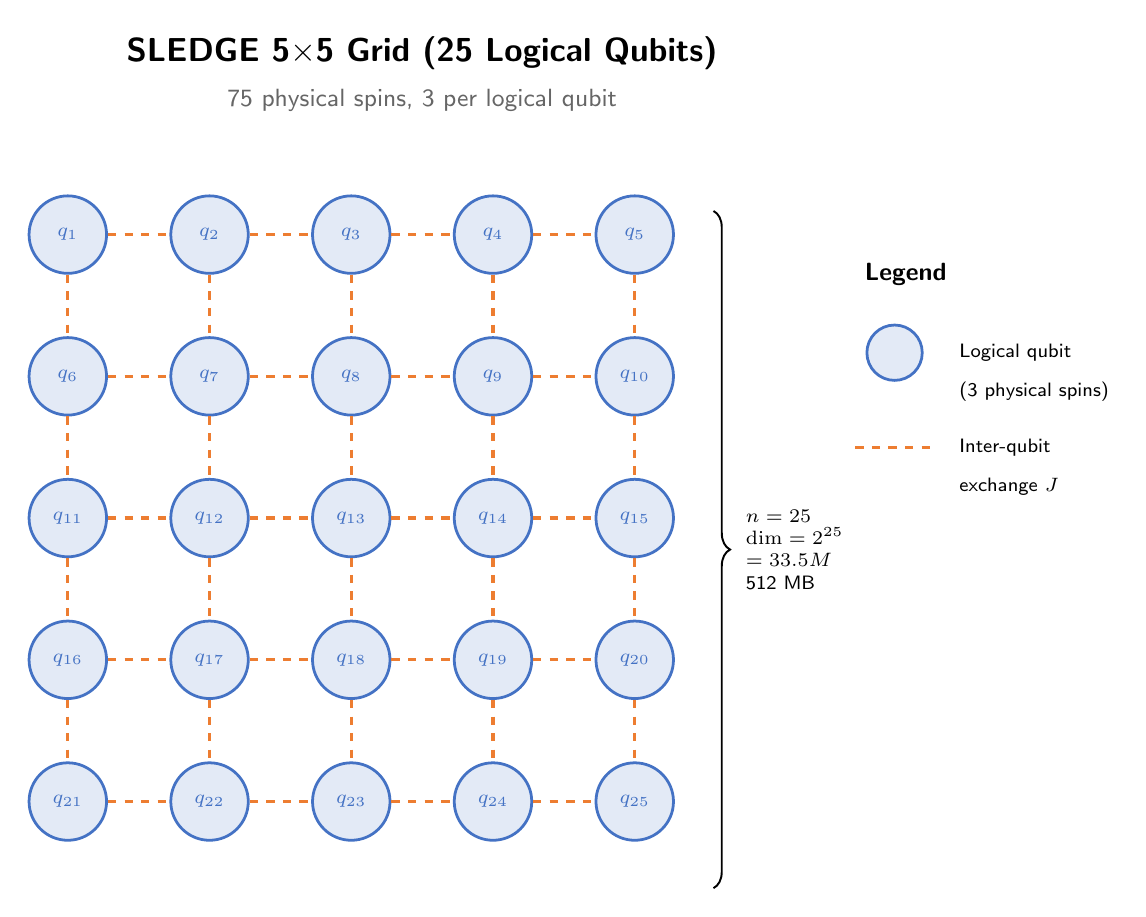
\begin{tikzpicture}[
    logqubit/.style={
        circle, draw=logblue, fill=logblue!15, minimum size=28pt,
        font=\sffamily\scriptsize\bfseries, text=logblue, line width=1pt
    },
    physpin/.style={
        circle, draw=physgray, fill=physgray!20, minimum size=6pt,
        inner sep=0pt, line width=0.5pt
    },
    intra/.style={
        -, line width=1pt, color=logblue!60
    },
    inter/.style={
        -, line width=1.2pt, color=exchinter, dashed
    }
]

% Title
\node[font=\sffamily\bfseries\large] at (4.5, 7.8) {SLEDGE 5$\times$5 Grid (25 Logical Qubits)};
\node[font=\sffamily\small, text=black!60] at (4.5, 7.2) {75 physical spins, 3 per logical qubit};

% Draw 5x5 grid of logical qubits
\foreach \row in {0,...,4} {
    \foreach \col in {0,...,4} {
        \pgfmathtruncatemacro{\qnum}{\row*5+\col+1}
        \node[logqubit] (q\row\col) at (\col*1.8, -\row*1.8 + 5.5) {$q_{\qnum}$};
        
        % Draw 3 tiny physical spins inside each logical qubit (below)
        % Skip for clarity - the logical qubit circle represents the triplet
    }
}

% Horizontal inter-qubit exchange couplings
\foreach \row in {0,...,4} {
    \foreach \col in {0,...,3} {
        \pgfmathtruncatemacro{\nextcol}{\col+1}
        \draw[inter] (q\row\col) -- (q\row\nextcol);
    }
}

% Vertical inter-qubit exchange couplings
\foreach \row in {0,...,3} {
    \foreach \col in {0,...,4} {
        \pgfmathtruncatemacro{\nextrow}{\row+1}
        \draw[inter] (q\row\col) -- (q\nextrow\col);
    }
}

% Legend
\node[font=\sffamily\small\bfseries, anchor=west] at (10, 5) {Legend};
\node[logqubit, minimum size=20pt] (legq) at (10.5, 4) {};
\node[font=\sffamily\scriptsize, anchor=west] at (11.2, 4) {Logical qubit};
\node[font=\sffamily\scriptsize, anchor=west] at (11.2, 3.5) {(3 physical spins)};

\draw[inter] (10, 2.8) -- (11, 2.8);
\node[font=\sffamily\scriptsize, anchor=west] at (11.2, 2.8) {Inter-qubit};
\node[font=\sffamily\scriptsize, anchor=west] at (11.2, 2.3) {exchange $J$};

% Annotations
\draw[decorate, decoration={brace, amplitude=6pt}, line width=0.7pt]
    (8.2, 5.8) -- (8.2, -2.8) node[midway, right=8pt, font=\sffamily\scriptsize, align=left] {
        $n = 25$\\$\dim = 2^{25}$\\$= 33.5\text{M}$\\512 MB
    };

\end{tikzpicture}
\end{document}
